\section{Introduction}\label{sec:intro}

\IEEEPARstart{T}{he} proliferation of edge intelligence and multimodal foundation models has spurred the deployment of edge-assisted Visual Question Answering (VQA) in mission-critical Internet-of-Things (IoT) and cyber-physical networks, including autonomous unmanned aerial vehicles (UAVs), remote environmental sensing, and robotic search-and-rescue~\cite{lobry2020rsvqa,zheng2024aerialee}. In these wireless scenarios, a battery-powered edge sensor captures high-resolution imagery and offloads visual data over an unreliable, fading wireless uplink to an edge computing node hosting a multi-billion-parameter Vision--Language Model (VLM)~\cite{wang2024qwen2vl,bai2025qwen25vl}. The edge VLM executes joint visual perception and natural language reasoning to respond to complex semantic queries in real time.

However, delivering high-accuracy VQA services over wireless networks encounters two severe, coupled bottlenecks:
\begin{enumerate}
    \item \textbf{Wireless Fading Outages and Channel Degradation}: Wireless channels are inherently subject to multipath fading, shadowing, and path loss. Under classical separate source-channel coding (SSCC) and block-length constrained digital codes such as low-density parity-check (LDPC) codes, channel attenuation triggers the notorious ``cliff effect''~\cite{bourtsoulatze2019djscc}. When channel conditions drop below the waterfall threshold, block decoding fails entirely, corrupting the bitstream and leading to catastrophic answer errors.
    \item \textbf{Multimodal Token Explosion and Edge Compute Costs}: Contemporary autoregressive VLMs divide input images into a fine-grained grid of visual patches, projecting them into lengthy sequences of visual tokens~\cite{wang2024qwen2vl}. The computational complexity of the Transformer self-attention mechanism scales quadratically with the visual sequence length, $\mathcal{O}(T_v^2)$~\cite{sabanovic2026inarvl}. For simple, coarse-grained semantic queries (e.g., verifying object presence), processing hundreds of redundant visual tokens imposes exorbitant computational and energy overhead on the edge server without tangible task accuracy improvement.
\end{enumerate}

\begin{figure*}[!t]
\centering
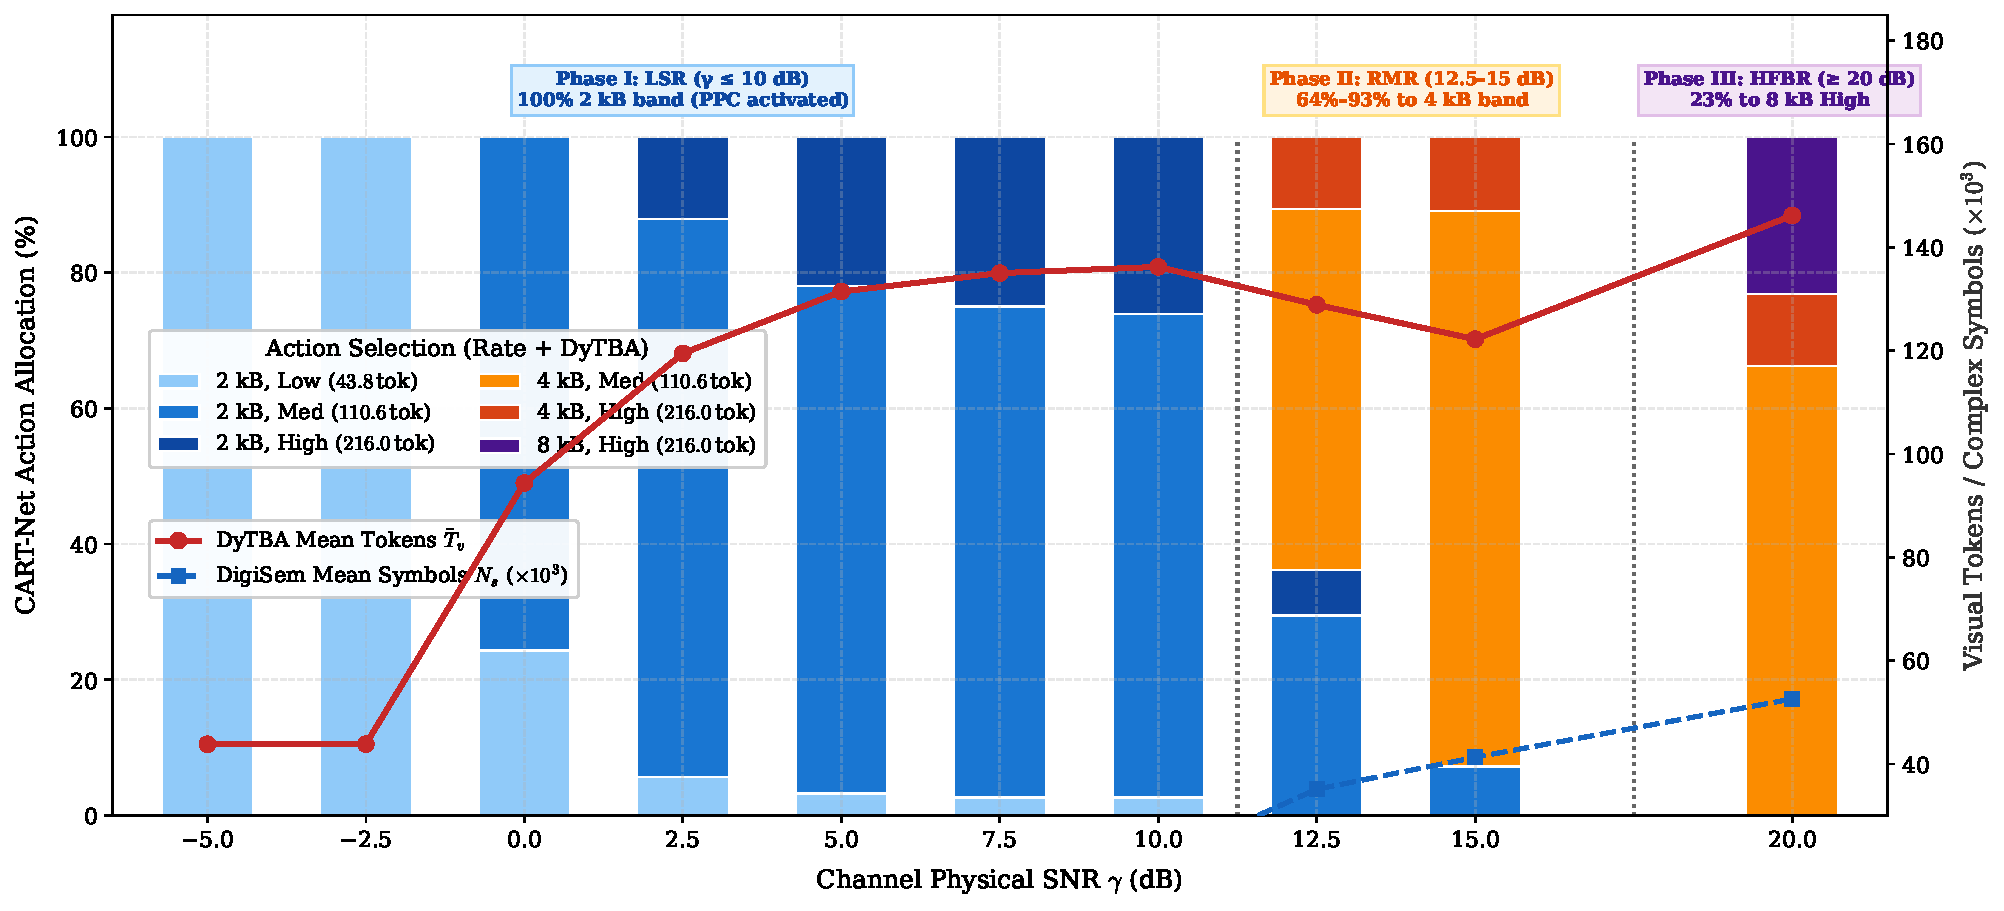
\includegraphics[width=0.98\linewidth]{figures/tgcn_publication_figures_20260922/fig2_dynamic_routing_architecture.pdf}
\caption{System framework and dynamic action routing of the proposed task-oriented cross-layer semantic communication system. (a) A lightweight transmitter-side policy inspects question text embeddings, an image spatial preview, and physical channel state information (CSI) $\gamma$, dynamically selecting an action $a \in \mathcal{A}$ spanning 3 source bitrates and 3 receiver visual token budgets. (b) Empirical routing distribution across 2,400 blind test images over Rician fading ($K=6\text{ dB}$), illustrating the emergent three-phase adaptation mechanics: Link Survival ($\le 10\text{ dB}$), Rate Migration ($12.5 \sim 15\text{ dB}$), and High-Fidelity Burst ($\ge 20\text{ dB}$).}
\label{fig:framework_overview}
\end{figure*}

To break through the Shannon capacity bottleneck, \emph{semantic communication} (SemCom) has emerged as a cornerstone of next-generation 6G communications~\cite{qin2021semantic,gunduz2023beyond}. Rather than seeking error-free bit reconstruction, task-oriented semantic communication extracts and conveys only task-relevant semantics. For multimodal reasoning, pioneer frameworks such as MU-DeepSC~\cite{xie2022mudeepscwcl,xie2021mudeepsc} and Goal-Oriented Scene-Graph communication~\cite{liu2024gosg} have successfully demonstrated the power of joint source-channel transceivers.

Nevertheless, translating existing semantic communication theories into practical wireless networks exposes critical design deficiencies:
\begin{itemize}
    \item \textbf{Reliance on Unquantized Analog Transmission}: The vast majority of existing SemCom paradigms (e.g., DeepJSCC and MU-DeepSC) rely on analog transmission, mapping latent neural features directly into continuous channel symbols without digital constellation mapping or error-correction framing. This assumption conflicts with standardized digital communication infrastructure (e.g., 3GPP LDPC, QPSK/16-QAM) and overlooks discrete packet erasure dynamics.
    \item \textbf{Neglect of Downstream Edge Inference Energy}: Existing works predominantly focus on reducing radio transmission bandwidth while evaluating toy-scale classification decoders (e.g., MCAN or 3-layer CNNs). In practical edge systems running 4B-to-7B parameter VLMs, the energy consumed by neural inference equals or surpasses radio transmission energy~\cite{zheng2024aerialee,auer2011howmuch}.
    \item \textbf{Rigid Physical Energy Trade-offs}: Conventional systems enforce static transmission parameters. In energy-constrained edge uplinks (e.g., battery-operated aerial sensors), transmitting a compact source payload over fewer channel symbols enables the transmitter to allocate higher energy per symbol. This unlocks a significant effective signal-to-noise ratio (SNR) boost that can shield the communication link from deep fading outages.
\end{itemize}

To address these challenges, this paper presents an end-to-end, cross-layer task-oriented semantic communication framework for edge VQA under realistic digital channel coding and Rician fading. As depicted in Fig.~\ref{fig:framework_overview}, the system features a deep variational neural image compression codec, a 3GPP 5G-compliant $\text{LDPC}(1020, 512)$ physical layer, and an edge-deployed Qwen3-VL-4B foundation model adapted via low-rank adaptation (LoRA)~\cite{hu2021lora,dettmers2024qlora}. A lightweight transmitter-side policy network dynamically co-optimizes the source bitrate $B \in \{2\text{k}, 4\text{k}, 8\text{k}\}$ bytes and the receiver visual token budget $T_v \in \{\mathrm{low}, \mathrm{medium}, \mathrm{high}\}$.

The primary contributions of this paper are summarized as follows:
\begin{enumerate}
    \item \textbf{Digital-Compatible Cross-Layer SemCom Architecture}: We propose an integrated semantic communication framework that couples deep variational source compression (CompressAI hyperprior) with standardized 3GPP digital channel coding ($\text{LDPC}(1020, 512)$) and a foundational VLM (Qwen3-VL-4B). This establishes a practical, digitally deployable semantic pipeline.
    \item \textbf{Dual-Mode Energy Formulation and Physical Layer Power Concentration}: We establish rigorous mathematical energy models encompassing both wireless transmission and edge VLM inference. We formulate two operational regimes: Mode~1 (constant symbol power) and Mode~2 (constant query energy budget). We prove that under Mode~2, transmitting a compact 2000-byte payload yields an exact $+3.01\text{ dB}$ (vs. 4000 bytes) and $+6.00\text{ dB}$ (vs. 8000 bytes) physical SNR boost, effectively circumventing the LDPC outage waterfall under harsh fading.
    \item \textbf{Channel-Aware Semantic Policy Network}: We design a lightweight multi-branch policy network mapping query semantic embeddings, image preview features, and instantaneous channel SNR into a 9-action discrete space. The policy exhibits an emergent three-phase adaptation: a \emph{Link Survival Regime} ($\le 10\text{ dB}$), a \emph{Rate Migration Regime} ($12.5 \sim 15\text{ dB}$), and a \emph{High-Fidelity Burst Regime} ($\ge 20\text{ dB}$).
    \item \textbf{Extensive Empirical Validation on TDIUC}: We evaluate our framework over 2,400 independent blind test images across 10 channel SNRs ($-5.0\text{ dB} \dots 20.0\text{ dB}$) under Rician fading ($K=6\text{ dB}$). Experimental results show that under harsh fading ($2.5\text{ dB}$, Mode 2), our policy achieves $36.92\%$ accuracy, delivering a $+29.92\%$ advantage over fixed 4k and a $+27.71\%$ advantage over channel-blind routing. Furthermore, the proposed policy strictly establishes the non-dominated Pareto frontier across RF energy, system latency, and task accuracy.
\end{enumerate}

The rest of this paper is structured as follows. Section~\ref{sec:related} discusses related work. Section~\ref{sec:system} presents the system model and cross-layer optimization problem. Section~\ref{sec:policy} describes the policy network architecture and its three-phase adaptation. Section~\ref{sec:experiments} provides extensive empirical evaluations and discussions. Finally, Section~\ref{sec:conclusion} concludes the paper.
